\section{Livello di applicazione}

\subsection{Princìpi delle applicazioni di rete}

\subsubsection{Architetture delle applicazioni di rete}
Lo sviluppatore di applicazioni deve progettare l'\textbf{architettura dell'applicazione} (\textit{application architecture}). Ci sono due tipi di architettura: \textbf{client-server} o \textbf{P2P (peer-to-peer)}.

L'\textbf{architettura client-server} si basa su un \textit{server} che sarà sempre attivo, con un indirizzo IP statico e sarà connesso con altri server, mentre il \textit{client} è colui che *inizia* la comunicazione con il server. Non succederà mai che il server proverà a contattare il client, e i client avranno degli indirizzi IP dinamici. Costi alti per via dell'installazione e manutenzione. Nel caso in cui il server cada e non sarà più raggiungibile tutta la rete cadrà, quindi abbiamo un \textbf{singolo punto di fallimento} che è il server.

L'\textbf{architettura P2P pura} si basa sulla comunicazione tra i vari \textit{peer}, dove ogni peer agisce sia come \textit{client} che come \textit{server}. Non esiste un \textit{host} sempre attivo. È un'architettura scalabile, poiché le risorse sono distribuite tra i vari peer, ma difficile da gestire per la sicurezza (tutti gli host devono essere protetti adeguatamente, se uno solo non è protetto tutta la rete è insicura) visto che manca un punto centrale di controllo, e ogni peer è un potenziale punto di fallimento.

Esiste un'architettura \textbf{ibrida}, quindi un mix di architettura client-server e P2P. Il server serve come mezzo di ricerca, fungendo da directory o tracker. I peer mandano una richiesta al server che la inoltra agli altri peer, mettendo poi in comunicazione i peer nella modalità P2P.

\subsubsection{Processi comunicanti}
Nei sistemi operativi i programmi prendono nome di \textbf{processi comunicanti}.
\begin{itemize}
    \item \textbf{Processo}: programma in esecuzione su un host. Più processi sullo stesso host comunicano tramite \textbf{schemi interprocesso}, mentre processi su host differenti comunicano tramite scambio di messaggi.
    \item \textbf{Processo client}: processo che dà inizio alla comunicazione.
    \item \textbf{Processo server}: processo che attende di essere contattato.
    \item \textbf{Socket}: Il processo comunica tramite un socket, un'interfaccia che mette in comunicazione il livello del processo applicativo e il livello trasporto. È equiparabile a una porta logica.
    \item \textbf{API}: Application Programming Interface, definisce come un'applicazione accede ai servizi di trasporto. È un'interfaccia di programmazione.
\end{itemize}

Le applicazioni con architettura P2P hanno sia processi client che server. Il progettista dell'applicazione può scegliere il protocollo di trasporto e alcuni parametri a livello di trasporto.

Per identificare il processo ricevente bisogna avere due informazioni:
\begin{itemize}
  \item \textbf{Indirizzo dell'host}: specificato dal loro \textbf{indirizzo IP}, un indirizzo logico di 32 bit che identifica univocamente l'host.
  \item \textbf{Identificatore del processo ricevente sull'host di destinazione}: la sua \textbf{socket}, il \textbf{numero di porta di destinazione} svolge questo compito, identificando un processo specifico sull'host.
\end{itemize}

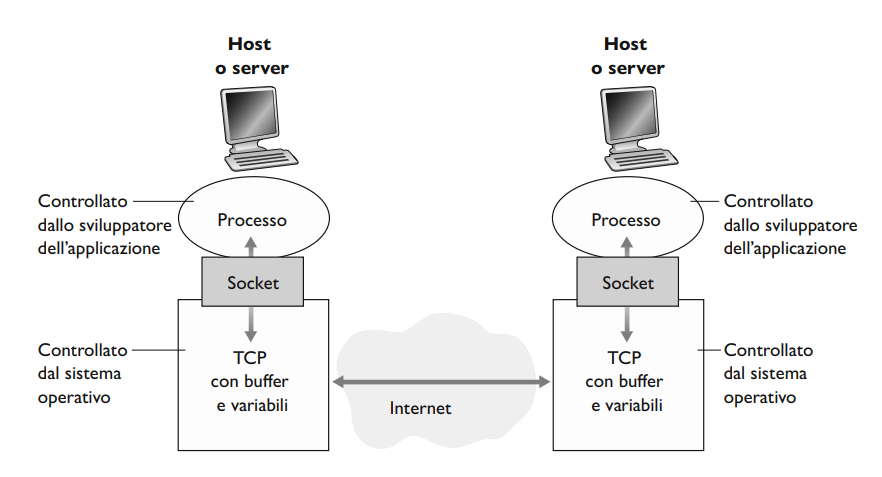
\includegraphics[width=\textwidth, height=6cm, keepaspectratio]{img/processi-socket.png}

\subsubsection{Servizi di trasporto disponibili per le applicazioni}
L'applicazione lato mittente trasmette i messaggi tramite la socket. Lato ricevente, il protocollo a livello di trasporto deve consegnare i messaggi alla socket del processo ricevente, fornendo una comunicazione *logica* tra le applicazioni.

Esistono vari servizi offerti dai protocolli a livello di trasporto, tra cui: trasferimento dati affidabile, throughput, temporizzazione e sicurezza.

\subsubsection*{Trasferimento dati affidabile}
Molte applicazioni hanno la necessità di ricevere ogni pacchetto che gli viene mandato, poiché la perdita di pacchetto potrebbe causargli dei danni, per esempio economici. Hanno bisogno di un protocollo con un servizio di consegna garantita dei dati, cioè il \textbf{trasferimento affidabile dei dati} (\textit{reliable data transfer}), che si ottiene tramite meccanismi come acknowledgment e ritrasmissione.

Se il protocollo a livello di trasporto fornisce questo servizio, il processo mittente manderà i dati sapendo che arriveranno tutti a destinazione.

Alcune applicazioni, per esempio quelle multimediali, accettano la possibilità di perdita di dati poiché preferiscono la maggiore velocità di trasmissione, si dicono \textbf{applicazioni che tollerano le perdite} (\textit{loss-tolerant applications}), ovvero applicazioni che possono tollerare una certa perdita di dati senza impatti significativi sulla loro funzionalità.

\subsubsection*{Throughput}
Garantire il servizio di \textbf{throughput} significa garantire una certa quantità di banda per il collegamento, ovvero una certa *velocità* con cui i dati vengono trasferiti. Queste applicazioni vengono chiamate \textbf{applicazioni sensibili alla banda} (\textit{bandwidth-sensible applications}), ovvero applicazioni che richiedono un throughput minimo *garantito*.

Esistono delle applicazioni che non hanno bisogno di una quantità di throughput garantita, ma sono elastiche, da qui il nome \textbf{applicazioni elastiche} (\textit{elastic applications}), ovvero applicazioni che si adattano al throughput disponibile in quell'istante.

\subsubsection*{Temporizzazione}
Per le applicazioni in tempo reale è necessaria una comunicazione quasi istantanea, hanno bisogno della garanzia che la trasmissione avvenga sotto un determinato tempo. Queste garanzie di temporizzazione sono spesso difficili da ottenere nella pratica.

\subsubsection*{Sicurezza}
Infine, un protocollo a livello di trasporto può garantire la sicurezza dei dati mediante, per esempio, la crittografia. I servizi di sicurezza possono includere confidenzialità, integrità e autenticazione.

\subsubsection{Servizi di trasporto offerti da Internet}
Esistono due protocolli di trasporto per le applicazioni di internet:
\begin{itemize}
  \item \textbf{TCP}: prevede una connessione e un trasporto affidabile dei dati.
    \textbf{Servizio orientato alla connessione} \textit{(connection-oriented service)}: fa in modo che client e server si scambino informazioni di controllo a livello di trasporto prima che i messaggi a livello di applicazione comincino a fluire. Questa procedura, denominata \textbf{handshaking}, stabilisce uno *stato* sia sul client che sul server, pre-allertandoli per lo scambio di messaggi.
    Dopo la fase di \textit{handshaking} si dice che esiste una \textbf{connessione TCP} tra le socket di client e host, una connessione di tipo \textit{full-duplex} (i processi possono scambiare messaggi contemporaneamente in entrambe le direzioni).
    \textbf{Servizio di trasferimento affidabile} \textit{(reliable data transfer service)}: il protocollo TCP garantisce ai processi il flusso di dati senza errori, utilizzando meccanismi come acknowledgment, ritrasmissione e numeri di sequenza.
    TCP evita la congestione della rete, *attivamente* strozzando il flusso quando è eccessivo.
  \item \textbf{UDP}: protocollo minimale, è "senza connessione" (non ha bisogno di \textit{handshaking}), ciò non garantisce l'affidabilità della connessione. UDP non garantisce la consegna, l'ordine o l'assenza di duplicati. Non ha un meccanismo di gestione della congestione, manda il flusso di dati al livello di rete a qualsiasi velocità, lasciando la gestione della congestione all'applicazione.
\end{itemize}

\subsubsection{Protocolli a livello di applicazione}
I protocolli a livello di applicazione devono stabilire:
\begin{itemize}
\item i tipi di messaggi scambiati (richiesta o risposta), definendo lo \textbf{scopo} del messaggio.
\item la sintassi dei vari tipi di messaggio, definendo il \textbf{formato} del messaggio.
\item la semantica dei campi, definendo il \textbf{significato} dei campi all'interno del messaggio.
\item le regole per regolare quando e come un processo invia e risponde ai messaggi, definendo la \textbf{sequenza} dei messaggi e le \textbf{azioni} intraprese dai processi comunicanti.
\end{itemize}

\subsection{Web e HTTP}
Il \textbf{Web} è \textit{on demand}, ciò significa che si può avere quello che si vuole quando si vuole, accedendo a risorse tramite \textbf{URL} \textit{(Uniform Resource Locator)}.

\subsubsection{Panoramica di HTTP}
\textbf{HTTP (\textit{HyperText Transfer Protocol})} è un protocollo a livello di applicazione \textit{request-response} che utilizza \textbf{TCP} come protocollo di trasporto, implementato a due programmi, client e server.
\textbf{Pagina web}: documento costituito da \textit{più} oggetti, un \textbf{oggetto} è un file indirizzabile tramite un \textbf{URL}.
In un \textit{URL} ci sono tre componenti: il protocollo (es. `http://`), il nome dell'host e il percorso dell'oggetto.
I \textbf{browser} implementano il protocollo \textit{HTTP} lato client, \textit{richiedendo} oggetti.
I \textbf{server web} implementano il protocollo \textit{HTTP} lato server (Apache è un esempio), \textit{fornendo} oggetti e saranno sempre attivi con un indirizzo IP statico.
\textit{HTTP} è un protocollo \textbf{senza memoria di stato} (\textit{stateless protocol}), ovvero i server HTTP non mantengono alcuna informazione sulle richieste passate dei client.

\subsubsection{Connesioni persistenti e non persistenti}
Si possono creare due tipi di connessioni:
\begin{itemize}
  \item \textbf{non persistenti}: ogni coppia richiesta e risposta deve essere inviata su una connessione TCP \textit{separata}. C'è un overhead nell'aprire una nuova connessione TCP per ogni coppia richiesta-risposta.
  \item \textbf{persistenti}: tutte le comunicazioni sono mandate sulla stessa connessione TCP (scelta di default per HTTP), riutilizzando la stessa connessione TCP e riducendo l'overhead.
\end{itemize}

\subsubsection*{HTTP con connessioni non persistenti}
Nelle \textit{connessioni non persistenti TCP} ogni connessione viene chiusa dopo l'invio dell'oggetto da parte del server, quindi ogni connessione trasporterà un solo messaggio di richiesta e solo uno di risposta.
Esistono browser che possono aprire più connessioni TCP parallelamente per velocizzare.
\textbf{Round-trip time (RTT)}: tempo impiegato da un pacchetto per viaggiare dal client al server e tornare al client. È una \textit{misura} della latenza di rete. Include i ritardi di propagazione, di accodamento nei router e nei commutatori intermedi e di elaborazione del pacchetto. \\ 
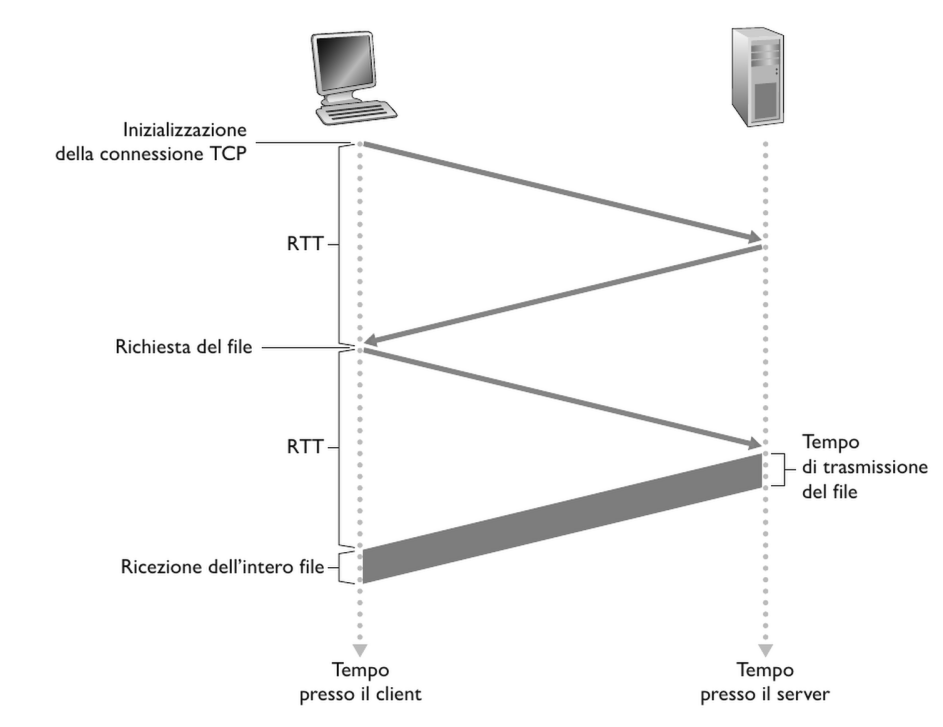
\includegraphics[width=\textwidth]{./img/rtt.png}
Quando un utente clicca su un collegamento ipertestuale il browser inizializza una connessione TCP con il web server, iniziando così un \textbf{handshake a tre vie} (three-way handshake): il client invia un piccolo segmento TCP al server (SYN), il server manda una conferma sempre con un piccolo segmento TCP (SYN-ACK), e il cliente manda una conferma di ritorno al server (ACK). Questo handshake serve a stabilire la connessione TCP.
Con queste prime due operazioni di handshake a tre vie calcoliamo il \textit{RTT}.
Il client ora invia un messaggio di richiesta HTTP insieme alla conferma di avvenuta ricezione (\textit{acknowledgement - ACK}), a messaggio ricevuto dal server il server procede a inviare il file al client. Il tempo di risposta totale sarà di 2 RTT (un RTT per l'handshake TCP e un RTT per la richiesta-risposta HTTP) più il tempo di trasmissione del file dal server al client.

\subsubsection*{HTTP con connessioni persistenti}
Nelle connessioni persistenti il server lascia aperta la connessione dopo la prima coppia di richiesta-risposta col client, tutte le altre coppie verranno trasmesse sulla stessa connessione, riutilizzando la stessa connessione TCP e riducendo l'overhead.
Una delle caratteristiche di queste connessioni è il \textit{pipelining}, la capacità di poter effettuare \textit{più} richieste senza aspettare la risposta delle richieste in corso.
La connessione si chiuderà dopo un lasso di tempo configurato in cui la connessione è stata inattiva.

\subsubsection{Formato dei messaggi HTTP}
Esistono due formati di messaggi HTTP per richiesta e risposta.

\subsubsection*{Messaggio di richiesta HTTP}
\begin{quote}
  GET /somedir/page.html HTTP/1.1 \newline
  Host: www.someurl.com \newline
  Connection: close \newline
  User-agent: Mozilla/5.0 \newline
  Accept-language: fr
\end{quote}

Questa è una richiesta HTTP, può avere un numero indefinito di righe, la riga fondamentale è la prima che è la \textbf{riga di richiesta}, le succesive sono \textbf{righe di intestazione}.
La riga di richiesta ha 3 campi: metodo (GET, POST, DATA, PUT, DELETE), l'URL e la versione di HTTP. \newline
\textbf{GET} è il metodo più utilizzato nel web, si usa per richiedere un oggetto tramite l'URL.
Notiamo la riga "Connection: close", con questa riga il browser comunica al server che non si deve occupare di connessioni eprsistenti, deve chiudere la connessione dopo aver iniviato l'oggetto.\newline
Alla fine del richiesta troviamo un \textit{corpo} del messaggio, vuoto in caso di metodo GET, utilizzato in caso di metodo POST. \newline
Il metodo \textbf{POST} viene utilizzato per mandare form compilati dell'utente al server, si può utilizzare anche il metodo GET per questo scopo ma includendo questi dati nell'URL della pagina richiesta. \newline
Il metodo \textbf{HEAD} viene utilizzato dagli sviluppatori, è come il metodo \textit{GET} ma si riceve solo la risposta HTTP, senza ricevere l'oggetto. \newline
Il metodo \textbf{PUT} viene utilizzato per caricare dal client dei file sul server. \newline
Il metodo \textbf{DELETE} viene utilizzato per cancellare file sul server (spesso disabilitato per ragioni di sicurezza insieme al metodo PUT). \newline

\includegraphics[width=\textwidth]{./img/richiestaHTTP.png}

\subsubsection*{Messaggio di risposta HTTP}
\begin{quote}
  HTTP/1.1 200 OK
  Connection: close \newline
  Date: Thu, 18 Aug 2015 15:44:04 GMT \newline
  Server: Apache/2.2.3 (CentOS) \newline
  Last-Modified: Tue, 18 Aug 2015 15:11:03 GMT \newline
  Content-Lenght: 6821 \newline
  Content-Type: text/html \newline
  (data data data data ....)
\end{quote}

Abbiamo: una \textbf{riga di stato} iniziale (contenente 3 campi, versione di protocollo, codice di stato HTTP e il corrispettivo messaggio), sei \textbf{righe di intestazione} e il \textbf{corpo dell'oggetto} finale (fulcro del messaggio, contiene l'oggetto richiesto). \newline
Esistono vari codici di stato, questi i più comuni:
\begin{itemize}
  \item \textbf{200 - OK}: la richiesta ha avuto successo e in risposta si invia l’informazione.
  \item \textbf{301 - Moved Permanently}: l’oggetto richiesto è stato trasferito in modo permanente; il nuovo URL è specificato nell’intestazione Location: del messaggio di risposta. Il client recupererà automaticamente il nuovo URL.
  \item \textbf{400 - Bad Request}: si tratta di un codice di errore generico che indica che la richiesta non è stata compresa dal server.
  \item \textbf{404 - Not Found}: il documento richiesto non esiste sul server.
  \item \textbf{505 - HTTP Version Not Supported}: il server non dispone della versione di protocollo HTTP richiesta.
\end{itemize}

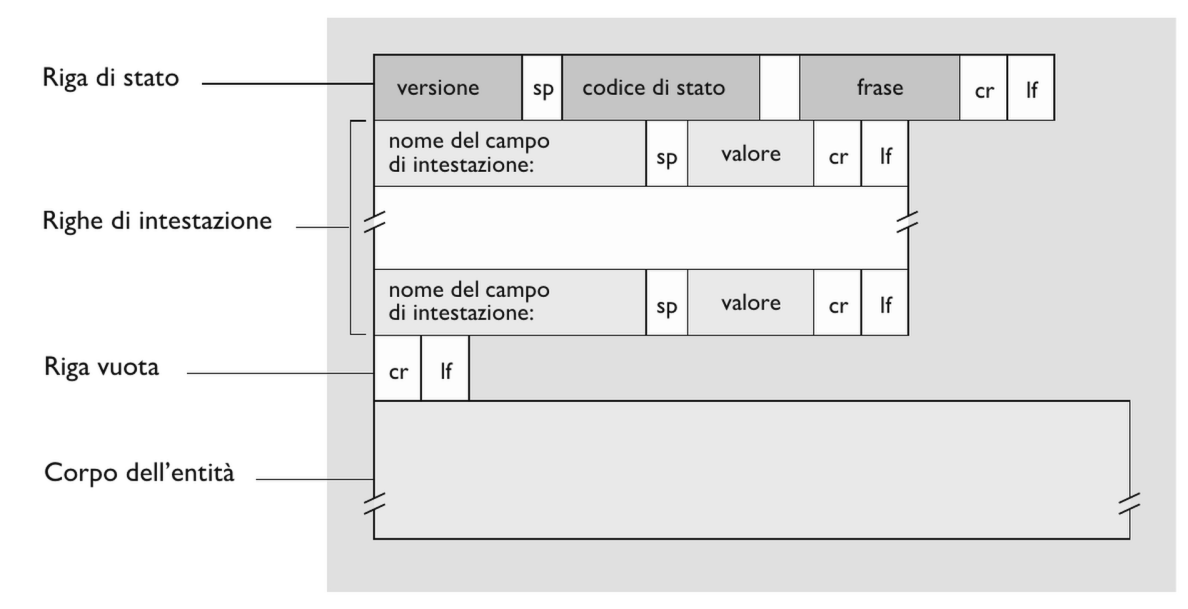
\includegraphics[width=\textwidth]{./img/rispostahttp.png}

\subsubsection{Cookie}
HTTP è un protocollo \textit{stateless}, un elemento utile per i webserver sono i \textbf{cookie}, un identificativo per l'utente che mantiene le informazioni sul server, per esempio l'\textit{autenticazione}.
È formato da 4 componenti, tra cui:
\begin{itemize}
  \item Riga di intestazione nel messaggio di risposta HTTP (Set-cookie: numero identificativo)
  \item Riga di intestazione nel messaggio di richeista HTTP (Cookie: numero identificativo)
  \item File cookie, mantenuto sul sistema terminale dell'utente e gestito dal browser del client
  \item Database sul webserver che mantiene l'identificativo dei cookie
\end{itemize}

\begin{quote}
  I cookie possono anche essere usati per creare un livello di sessione utente al di sopra di HTTP che è privo di stato.
\end{quote}

\subsubsection{Web caching (proxy server)}

\subsection{Posta elettronica}
Mezzo di comunicazione asincrono, tre componenti principali: gli \textbf{user agent} (o agenti utente), i \textbf{mail server} (server di posta) e il \textbf{protocollo SMTP (Simple Mail Transfer Protocol)}. 
L'\textit{user agent} invia il messaggio al proprio \textit{mail server} (il distributore del servizio) che invierà la mail al \textit{mail server} del destinatario.
Componenti della posta elettronica:
\begin{itemize}
  \item \textbf{casella di posta}: contenitore dei messaggi in arrivo, collocata in un \textit{mail server}.
  \item \textbf{Coda di messaggi}: mail che devono arrivare al destinatario.
  \item \textbf{Protocollo SMTP} (Simple Mail Transfer Protocol): regola la comunicazione tra i \textit{mail server} e tra gli \textit{user agent} e i proprio \textit{mail server}. Principale protocollo a livello di applicazione per la posta elettronica, utilizza \textit{TCP}.
  \begin{quote}
    Quando un server invia posta a un altro, agisce come client SMTP; quando invece la riceve, funziona come server SMTP.
  \end{quote}
\end{itemize}

\subsubsection{SMTP}
Utilizzo di TCP, utilizza la \textbf{porta 25}, è un \textit{protocollo con stato}, codificato in ASCII-7bit. \newline
Si prevedono 3 fasi diverse:
\begin{itemize}
  \item Prima fase: handshake
  \item Seconda fase: scambio effettivo dei messaggi
  \item Terza fase: chiusura della connessione 
\end{itemize}

\subsubsection*{Scenario di funzionamento del protocollo}
\begin{enumerate}
  \item L'user agent mittente compone l'indirizzo mail del destinatario
  \item L'user agent invia il messaggio al mail server del mittente
  \item Il mail server mittente apre una connessione TCP con il mail server del destinatario sulla porta 25
  \item Il client SMTP (mail server mittente) invia il messaggio tramite la connessione TCP e lo colloca nella coda dei messaggi
  \item Il mail server del destinatorio invia il messaggio nella mail box
  \item L'user agent destinatario può ora leggere il messaggio
\end{enumerate}

\includegraphics[width=\textwidth]{./img/smtp.png}

Si utilizzano dei mail server poiché nel caso in cui le mail non possono essere consegnate in un preciso momento o ci sono errori, il mail server può fare vari tentativi (in base alla configurazione fatta) per consegnare il messaggio.

continuo su tablet, pc scarico. inserire schema + appunti.

\subsubsection{Protocolli di accesso alla posta}

\subsection{DNS}
Il \textbf{DNS} è un protocollo, ma in realtà è un sistema, \textit{Domain Name System}.
Il web è identificato da un nome simbolico, il nome dell'host, ma il modo univoco per identificare il server è il suo indirizzo ip (32 Byte).
È un sistema distribuito, esistono vari server che conoscono l'associazione fra nome host e indirizzo IP. \newline
È un protocollo a livello di applicazione, i vari servizi che offre sono:
\begin{itemize}
  \item Traduzione degli hostname in indirizzi IP.
  \item Host aliasing, più nomi per lo stesso indirizzo ip (stesso host). Esiste un \textbf{nome canonico} della macchina che la identifica, esistono anche degli \textbf{alias} che sono altri nomi per la stessa macchina.
  \item Possibilità di gestire la posta elettronica in server diversi ma con lo stesso hostname (esempio mail@unipa.it e unipa.it).
  \item Possibilità di distribuire il carico, più macchine possono gestire lo stesso server, ci saranno pìù server (e più indirizzi IP) per un unico hostname.
\end{itemize}

Non dobbiamo centralizzare il DNS in un unico server per evitare un \textit{single point of secure}, non è scalabile, scarsa manutenzione e difficoltà nel gestire il volume di traffico.

\subsubsection{Gestione gerarchica DNS}
Abbaimo un sistema gerarchico, più in alto abbiamo i \textbf{server radice}, sotto i \textbf{server TLD (top-level domain)} e infine i server \textbf{autoritativi (o di competenza)}. \newline
I \textit{server autoritativi} sono i server che posseggono le traduzioni, sono di società che posseggono host Internet, devono fornire i record DNS di pubblico dominio che mappano i nomi di tali host in indirizzi IP. \newline
I \textit{server TLD} sono responsabili dei domini ad alto livello (.com, .co.uk, .it\dots), vengono gestiti da nazioni o da aziende. \newline
I \textit{server radice} responsabile di tutto. Sono 13 nel mondo (numero limitato), verrà contattato da un \textbf{DNS locale} \newline
Il client contatterà sempre il server radice, che darà indicazioni su dove trovare i server TLD interessati che diranno al client qual'è il server autoritativo responsabile per l'hostname scelto.

\subsubsection{DNS locale}
Una macchina fuori la gerarchia, che si occuperà di fare da client per le comunicazioni da il client reale e l'host radice, funzionamento di intermediario.
Ogni ISP ha un \textbf{DNS locale} e lui opera da proxy, inoltra la query in una gerarchia di server D e lui opera da proxy, inoltra la query in una gerarchia di server DNS.
Approccio con \textbf{expiring date} per il mantenimento delle informazioni.

\subsubsection*{Esempio di query iterativa}
\begin{enumerate}
\item Il \textbf{client web richiedente} chiede al \textbf{client DNS proprio} (chiamata API del sistema) di tradurre un hostname.
\item Il \textbf{client DNS} parla col \textbf{server DNS locale}.
\item Il \textbf{server DNS locale} richiede informazioni al \textbf{server DNS radice}. 
\item Il \textbf{server DNS radice} da informazioni sul \textbf{server TLD} che avrà l'informazione richiesta al \textbf{server DNS locale}.
\item Il \textbf{server DNS locale} richiede informazioni al \textbf{server DNS TLD}. 
\item Il \textbf{server DNS TLD} darà informazioni sul \textbf{server di competenza} che conterrà l'informazione che ci interessa al \textbf{server DNS locale}. 
\item Il \textbf{server DNS locale} richiede informazioni al \textbf{server di competenza}. 
\item Il \textbf{server di competenza} darà l'IP corrispondente dell'hostname al \textbf{server DNS locale}.
\item Il \textbf{server DNS locale}, ricevendo l'informazione dal \textbf{server di competenza}, la manda al \textbf{client dns richidenete} che trasferirà l'informazione al \textbf{client web richiedente} che potrà accedere ora al \textbf{server web richiesto}.
\end{enumerate}

\subsubsection{Record DNS}
Formato \textbf{RR (Record di risorsa)}: (name, value, type, ttl). \newline
4 tipi di type:
\begin{itemize}
  \item \textbf{Type=A}: name = nome host, value = indirizzo IP
  \item \textbf{Type=NS}: name = dominio, value = nome del server di competenza
  \item \textbf{Type=CNAME (canonical name)}: name = \textit{nome alias} di un nome \textit{nome canonico}, value = \textit{nome canonico}
  \item \textbf{Type=MX}: value = nome del server di posta di \textit{name}, name = nome server
\end{itemize}

\subsubsection*{Esempio popolazione DB server}

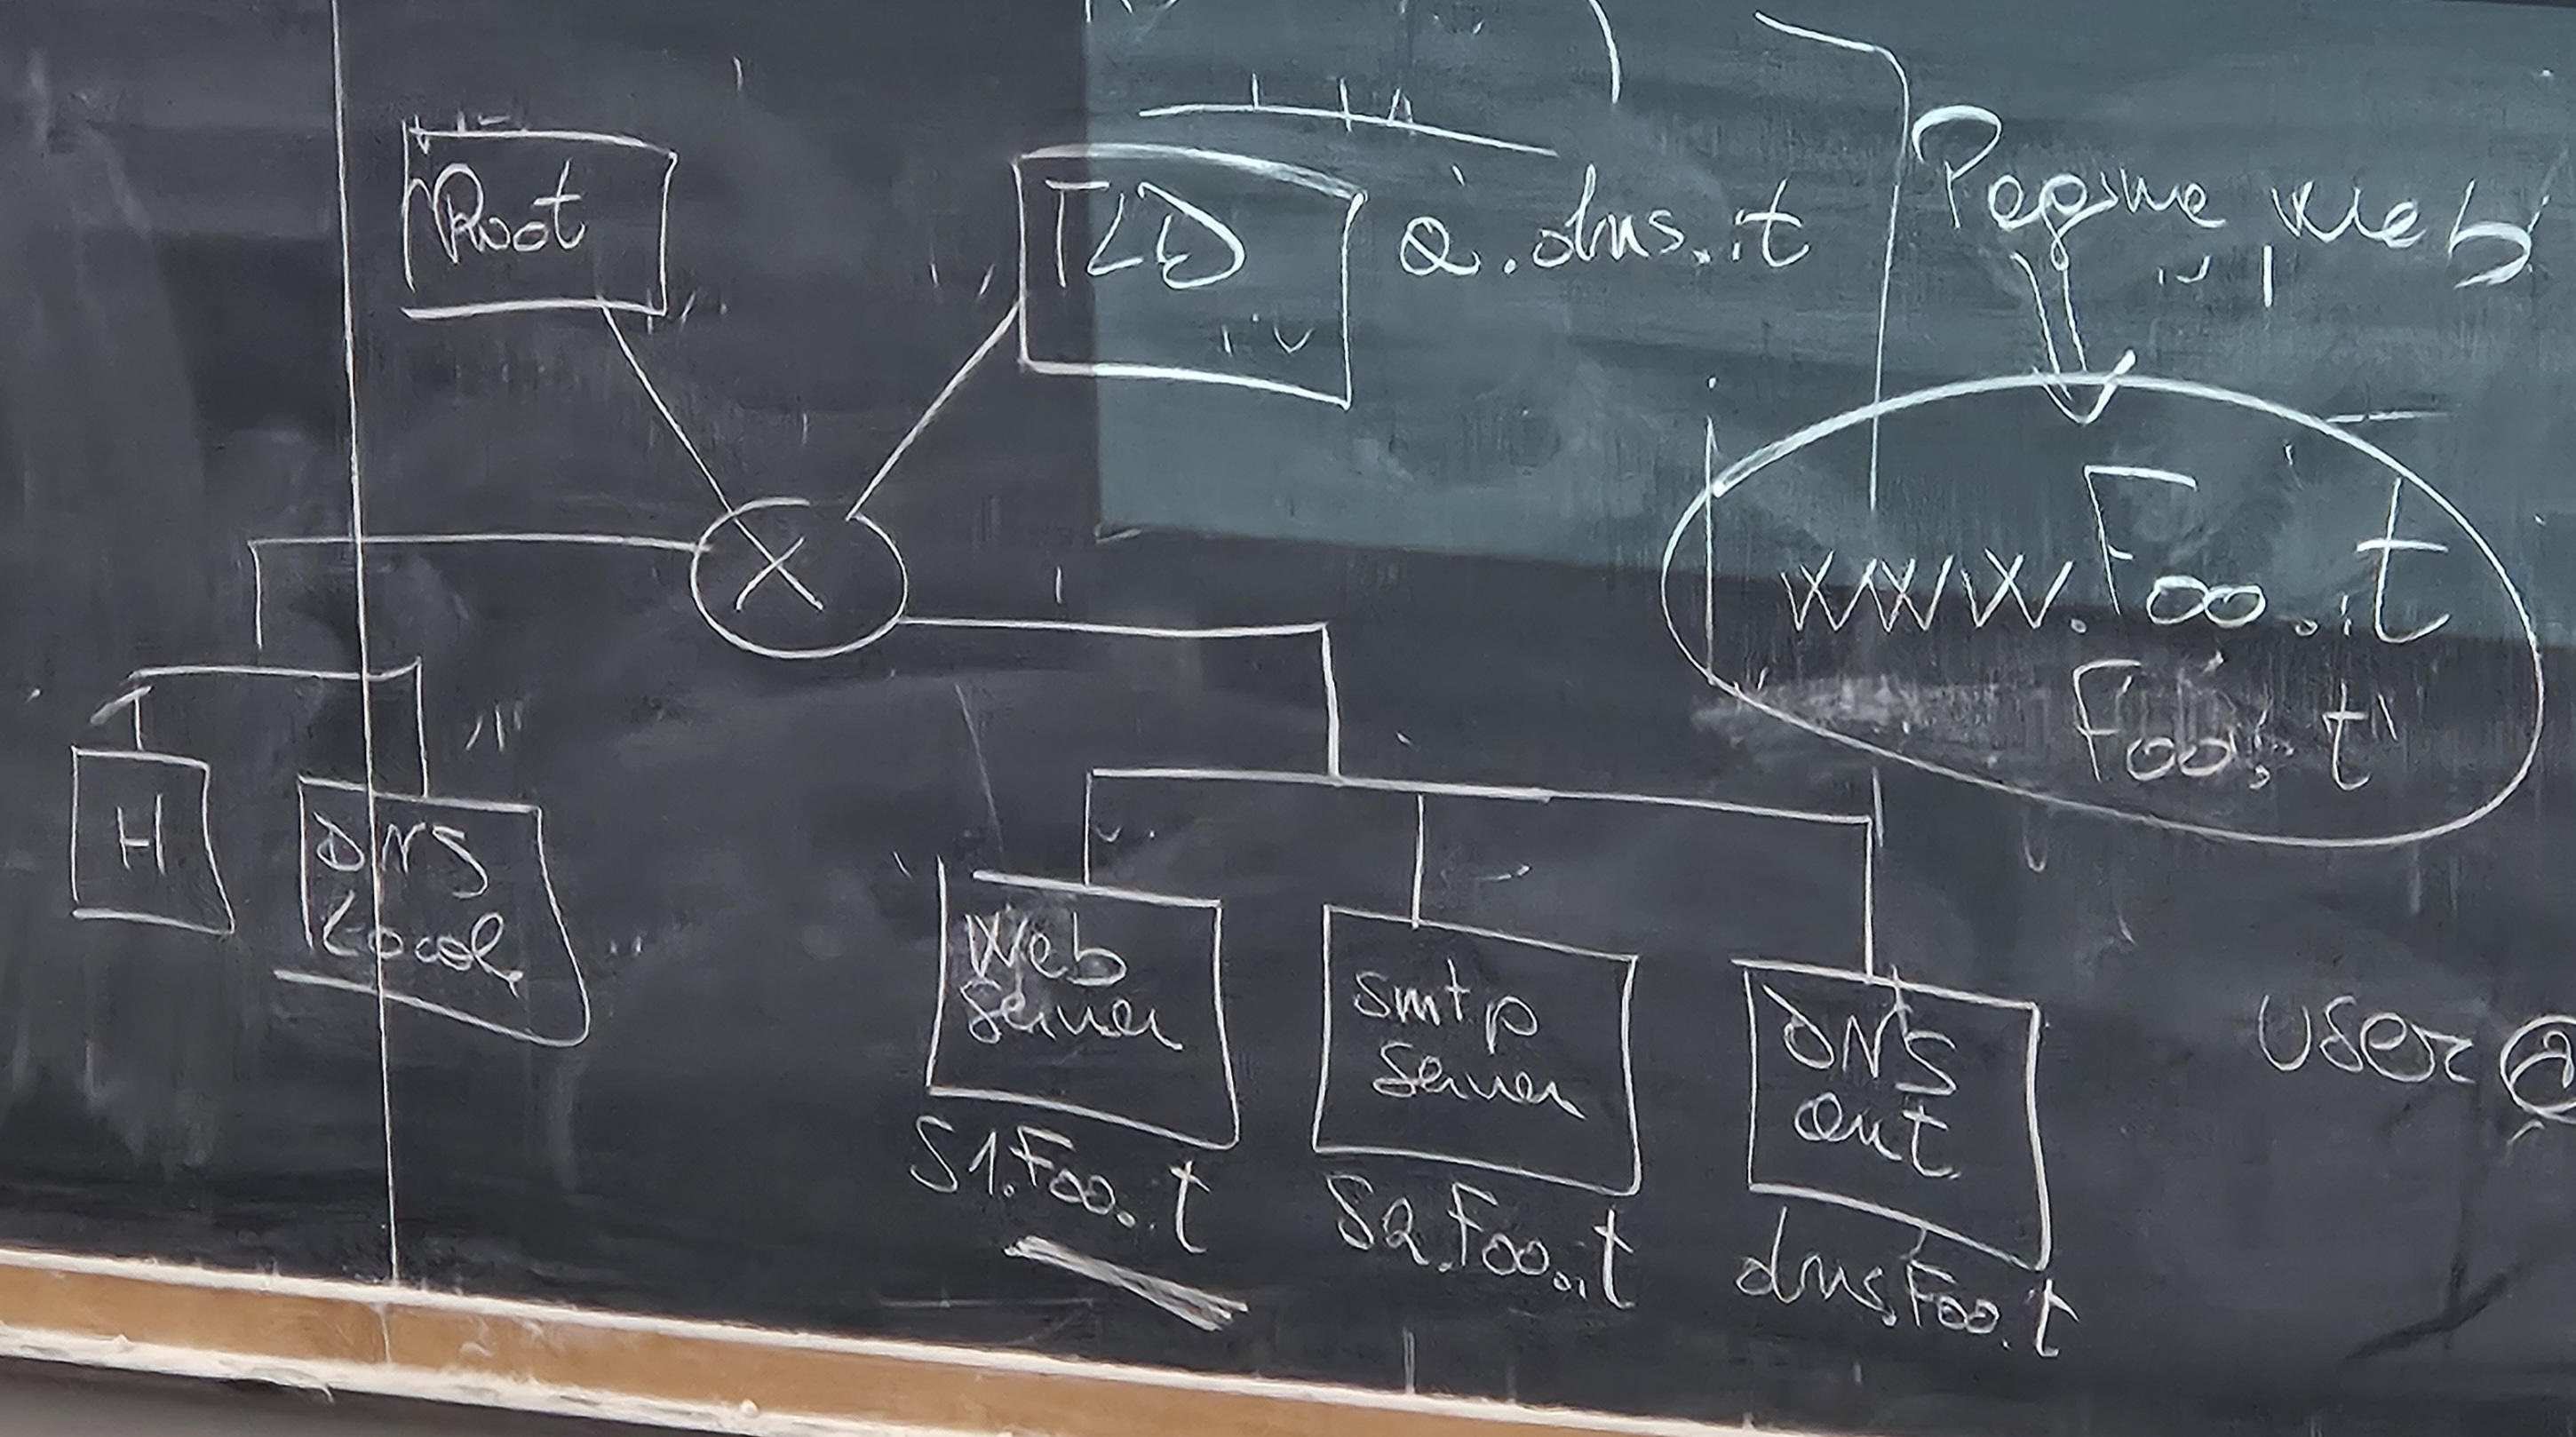
\includegraphics[width=\textwidth]{./img/dbdns.jpg} \\

\bigskip
\textbf{DB del server Radice} \newline
\begin{tabular}{lll}
\textbf{Name} & \textbf{Value} & \textbf{Type} \\
.it           & a.dns.it       & NS            \\
a.dns.it      & 22.4.9.10      & A             
\end{tabular}

\bigskip
\textbf{DB del server TLD} \newline
\begin{tabular}{lll}
\textbf{Name} & \textbf{Value}     & \textbf{Type} \\
foo.it        & dns.foo.it         & NS            \\
dns.foo.it    & 147.163.2.1        & A             
\end{tabular}

\bigskip
\textbf{DB del server DNS autoritativo} \newline
\begin{tabular}{lll}
\textbf{Name} & \textbf{Value}     & \textbf{Type}  \\
www.foo.it    & s1.foo.it          & CNAME          \\
foo.it        & s1.foo.it          & CNAME          \\
s1.foo.it     & 143.163.2.2        & A              \\
foo.it        & s2.foo.it          & MX             \\
s2.foo.it     & 143.163.2.3        & A              
\end{tabular}

\subsubsection{Messaggi DNS}
Il \textbf{protocollo DNS} mantiene lo stesso formato per le domande (query) e messaggi di risposta. 

